\chapter{Implementation strategies: evaluation and results}
\chaptermark{Implementation strategies: evaluation and results}
\label{chapter:exp_setup_results}
\minitoc

%%%%%%%%%%%%%%%%%%%%%%%%%%%%%%%%%%%%%%%%%%%%%%%%%%%%%%%%%%%%%%%%%%%%%%%%%%%%%%%%%%%%%%%%%%%%%%%
\section{Introduction}
The previous chapter presented two countermeasures against fault injection attacks and taking into account simple fault models, such as \textit{single-bit flip inside one register at a given clock cycle}. These countermeasures have been implemented by grouping the different DIFT-related registers in order to minimise the number of parity and redundancy bits. However, nowadays, studies~\cite{CGVCBLC-22-cardis,VDSPB-24-jce} have shown that is it possible to fault multiple bits precisely.

In this chapter, we present four different implementation's strategies of countermeasures to better protect the D-RI5CY mechanism against more complex fault models. Then, we evaluate each of these strategies in terms of security against more complex fault models. Finally, we compare them in terms of performance and area overhead. We implemented the minimisation of redundancy bits strategy in the last chapter. As shown in Chapter~\ref{chapter:countermeasures}, Hamming Code or even SECDED is better to use than just the simple parity for the correction and detection capacity. Hence, in this chapter, we do not implement others strategies for the simple parity protection. However, we present the results obtained from our simulations campaigns on the fault models considered in this chapter.

Section~\ref{section:chap6_faultmodels} introduces the different fault models considered.
Section~\ref{section:chap6_implem_strategies} introduces the four different strategies developed and assessed in this chapter.
Section~\ref{section:chap6_evaluation} presents the security assessment of these four strategies by giving the results associated to each fault model and the use cases to each strategy, and evaluate them in terms of security, performance, and area overhead.
Finally, in Section~\ref{section:chap6_discussion}, we discuss the results obtained from these five strategies according to their performance and area overhead and give the limitations for each strategy.

%%%%%%%%%%%%%%%%%%%%%%%%%%%%%%%%%%%%%%%%%%%%%%%%%%%%%%%%%%%%%%%%%%%%%%%%%%%%%%%%%%%%%%%%%%%%%%%
\section{Fault models considered in this chapter}
\label{section:chap6_faultmodels}
In Chapter~\ref{chapter:countermeasures}, we presented the results of fault injection campaigns targeting \textit{a single bit-flip in one register at a given clock cycle}, and \textit{a single bit-flip in two registers at two distinct clock cycles}. We demonstrated that lightweight countermeasures, such as simple parity, Hamming Code, or SECDED version of Hamming Code, are effective in protecting our DIFT mechanism against single bit-flips occurring in one register at one clock cycle or in two registers at two distinct clock cycles.

In this chapter, we extend our analysis to consider an attacker capable of injecting faults into DIFT-related registers, leading to a \textit{single bit-flip in two registers at a given clock cycle}. Furthermore, we account for an attacker able to induce \textit{multi-bit faults in one register at a given clock cycle}, as well as, \textit{multi-bit faults in two registers at a given clock cycle}. These fault models, introduced in Chapter~\ref{chapter:fissa}, are exhaustively tested across registers ranging from 1-bit to 10-bit. Registers larger than 10 bits, such as the configuration registers TPR and TCR, are excluded due to their size. For instance, simulating an exhaustive attack on a single 32-bit register for one cycle would require $2^{32}$ simulations (i.e: \powerTwo{pow(32,2)}{0} simulations), and for two 32-bit registers, the number of simulations would reach $2^{32} \times 2^{32}$ which is too large to be simulated in a reasonnable time. However, it is worth noting that the biggest register after these two 32-bit registers is a 6-bit register (cf. Tables~\ref{tab:strategy_2_groups}, \ref{tab:strategy_3_groups}, \ref{tab:strategy_4_groups}, \ref{tab:strategy_5_groups}, and \ref{tab:strategies_register_info}), so we fault every 1-bit to 6-bit registers.

The three fault models are exhaustively simulated across all possible values of these registers. To meet this objective, any DIFT-related register that maintains a 1-bit tag value, drives tag propagation or tag update processes, or holds security policy configurations, can be targeted. Additionally, registers storing redundancy bits for protection mechanisms are also considered.

% %%%%%%%%%%%%%%%%%%%%%%%%%%%%%%%%%%%%%%%%%%%%%%%%%%%%%%%%%%%%%%%%%%%%%%%%%%%%%%%%%%%%%%%%%%%%%%%
\section{Implementation strategies}
\label{section:chap6_implem_strategies}

Assessing the robustness of DIFT against more complex fault models requires comprehensive strategies that can identify vulnerabilities to enhance the system integrity. This section introduces four distinct strategies aimed at evaluating and enhancing the security of DIFT mechanisms against complex fault models. Each strategy offers a unique perspective on detecting, mitigating, or preventing the effects of multi bit-flip faults, contributing to a holistic approach in fortifying DIFT systems. By exploring these methodologies, we aim to provide actionable insights for developing more resilient DIFT solutions thanks to lightweight countermeasures.

\subsection{Strategy 2: Pipeline Stage Register Coupling for Robust Error Mitigation}

In the second implemented strategy, we rely on protecting each pipeline stage of our processor individually. To achieve this implementation, we decided to form seven groups: Instruction Fetch (IF) Stage, Instruction Decode (ID) Stage, Register File Tag, Execute (EX) Stage, two groups for the two registers TPR and TCR containing the security policy, and a last group with the Load/Store Unit. 

Table~\ref{tab:strategy_2_register_info} represents the different DIFT-related registers with their associated group.
Table~\ref{tab:strategy_2_groups} represents the number of protected bits inside each pipeline stage and their associated number of redundancy and parity bits, in the case of when SECDED is used. As depicted in this table, the number of protected bits differs a lot depending on the pipeline stage, ranging from one bit to thirty-two bits.
Otherwise, the HDL implementations are the same than Chapter~\ref{chapter:countermeasures} with two proposed implementations (see Figure~\ref{fig:implementation_sd_1} and Figure~\ref{fig:implementation_sd_2}). This strategy protects 107 bits by adding 30 redundancy bits and 7 parity bits which led to approximatively a 30\% increase in number of bits stored into registers.

\begin{table}[t]
    \centering
    \footnotesize
    \caption{D-RI5CY Registers Details List for Strategy 2}
    \label{tab:strategy_2_register_info}
    % \setlength{\tabcolsep}{5pt}
    \begin{tabular}{@{}rccc@{}}
        \toprule
        Register Name                   & Module                                & Size   & \tableTwoLines{Strategy}{2} \\\midrule
        pc\_id\_o\_tag                  & \textcolor{red}{Instruction}          & 1      & Gr1                         \\
        pc\_if\_o\_tag                  & \textcolor{red}{Fetch Stage}          & 1      & Gr1                         \\\hdashline
        alu\_operand\_a\_ex\_o\_tag     &                                       & 1      & Gr2                         \\
        alu\_operand\_b\_ex\_o\_tag     &                                       & 1      & Gr2                         \\
        alu\_operand\_c\_ex\_o\_tag     &                                       & 1      & Gr2                         \\
        alu\_operator\_o\_mode          &                                       & 2      & Gr2                         \\
        check\_d\_o\_tag                &                                       & 1      & Gr2                         \\
        check\_s1\_o\_tag               &                                       & 1      & Gr2                         \\
        check\_s2\_o\_tag               & \textcolor{blue}{Instruction}         & 1      & Gr2                         \\
        is\_store\_post\_o\_tag         & \textcolor{blue}{Decode Stage}        & 1      & Gr2                         \\
        memory\_set\_o\_tag             &                                       & 1      & Gr2                         \\
        regfile\_alu\_waddr\_ex\_o\_tag &                                       & 5      & Gr2                         \\
        register\_set\_o\_tag           &                                       & 1      & Gr2                         \\
        store\_dest\_addr\_ex\_o\_tag   &                                       & 1      & Gr2                         \\
        store\_source\_ex\_o\_tag       &                                       & 1      & Gr2                         \\
        use\_store\_ops\_ex\_o          &                                       & 1      & Gr2                         \\\hdashline
        rf\_reg[0]                      &                                       & 1      & Gr3                         \\
        rf\_reg[1]                      &                                       & 1      & Gr3                         \\
        rf\_reg[2]                      & \textcolor{LimeGreen}{Register File}  & 1      & Gr3                         \\
        \ldots                          & \textcolor{LimeGreen}{Tag}            & \ldots & Gr3                         \\
        rf\_reg[30]                     &                                       & 1      & Gr3                         \\
        rf\_reg[31]                     &                                       & 1      & Gr3                         \\\hdashline
        rs1\_o\_tag                     & \textcolor{DarkOrange}{Execute Stage} & 1      & Gr4                         \\\hdashline
        tcr\_q                          & \textcolor{DarkRed}{Control and}      & 32     & Gr5                         \\
        tpr\_q                          & \textcolor{DarkRed}{Status Registers} & 32     & Gr6                         \\\hdashline
        data\_type\_q\_tag              &                                       & 2      & Gr7                         \\
        data\_we\_q\_tag                & \textcolor{magenta}{Load/Store}       & 1      & Gr7                         \\
        rdata\_offset\_q\_tag           & \textcolor{magenta}{Unit}             & 2      & Gr7                         \\
        rdata\_q\_tag                   &                                       & 4      & Gr7                         \\
        \bottomrule
    \end{tabular}
\end{table}

\begin{table}[t]
    \centering
    \footnotesize
    \caption{DIFT-related protected registers -- Strategy 2}
    \label{tab:strategy_2_groups}
    \begin{tabular}{@{}rccccc@{}}
        \toprule
                & Protected stage          & \tableTwoLines{Number of}{bits} & \tableTwoLines{Number of}{protected bits} & \tableTwoLines{Number of}{redundancy bits} & \tableTwoLines{Number of}{parity bits} \\ \midrule
        Group 1 & Instruction Fetch Stage  & 2                               & 2                                         & 3                                          & 1                                      \\
        Group 2 & Instruction Decode Stage & 19                              & 19                                        & 5                                          & 1                                      \\
        Group 3 & Register File Tag        & 32                              & 32                                        & 6                                          & 1                                      \\
        Group 4 & Execute Stage            & 1                               & 1                                         & 2                                          & 1                                      \\
        Group 5 & TCR                      & 32                              & 22                                        & 5                                          & 1                                      \\
        Group 6 & TPR                      & 32                              & 22                                        & 5                                          & 1                                      \\
        Group 7 & Load/Store Unit          & 9                               & 9                                         & 4                                          & 1                                      \\ \midrule
        Total   &                          & 127                             & 107                                       & 30                                         & 7                                      \\
        \bottomrule
    \end{tabular}
\end{table}

\subsection{Strategy 3: Individual Register Encapsulation for Robust Error Mitigation}

In the third implementation strategy, we aim to enhance protection for every register associated with the DIFT within our processor. To achieve this, we categorised the registers into 24 specific groups, ensuring a more targeted and effective protection mechanism. The grouping was done based on each of them. Specifically, two groups were formed in the IF stage, addressing the initial handling of PC addresses. A significant portion, fourteen groups, was allocated to the ID stage, as this stage contains processing and handling of tags information. Additionally, one group was dedicated to the Register File Tag, as we consider this Register File as one register even if it is 32 registers to avoid an increase overhead for the Register File. For the EX stage, we formed a single group. Furthermore, two separate groups were created for the TPR and TCR registers, recognising their distinct control functions. Finally, four groups were designated for the Load/Store Unit, as it can be considered as the fourth stage of our processor. This structure allows for a granular protection approach, ensuring that each aspect of the processor's DIFT-related registers is securely managed. The issue with this strategy is the use of two redundancy bits and one parity bit to protect only one register bit.

Table~\ref{tab:strategy_3_register_info} represents the group composition with the different DIFT-related registers.
Table~\ref{tab:strategy_3_groups} represents the number of protected bits inside each protected group and their associated number of redundancy and parity bits, when SECDED is used. As depicted in this table, there is mainly only one bit protected in the majority of groups (16 groups over 24). This strategy protects 107 bits by adding 64 redundancy bits and 24 parity bits which led to approximatively a 70\% increase in number of bits stored into registers.

\begin{table}[t]
    \centering
    \footnotesize
    \caption{D-RI5CY Registers Details List for Strategy 3}
    \label{tab:strategy_3_register_info}
    % \setlength{\tabcolsep}{5pt}
    \begin{tabular}{@{}rccc@{}}
        \toprule
        Register Name                   & Module                                & Size   & \tableTwoLines{Strategy}{3} \\\midrule
        pc\_if\_o\_tag                  & \textcolor{red}{Fetch Stage}          & 1      & Gr1                         \\
        pc\_id\_o\_tag                  & \textcolor{red}{Instruction}          & 1      & Gr2                         \\\hdashline
        alu\_operand\_a\_ex\_o\_tag     &                                       & 1      & Gr3                         \\
        alu\_operand\_b\_ex\_o\_tag     &                                       & 1      & Gr4                         \\
        alu\_operand\_c\_ex\_o\_tag     &                                       & 1      & Gr5                         \\
        alu\_operator\_o\_mode          &                                       & 2      & Gr6                         \\
        check\_d\_o\_tag                &                                       & 1      & Gr7                         \\
        check\_s1\_o\_tag               &                                       & 1      & Gr8                         \\
        check\_s2\_o\_tag               & \textcolor{blue}{Instruction}         & 1      & Gr9                         \\
        is\_store\_post\_o\_tag         & \textcolor{blue}{Decode Stage}        & 1      & Gr10                        \\
        memory\_set\_o\_tag             &                                       & 1      & Gr11                        \\
        regfile\_alu\_waddr\_ex\_o\_tag &                                       & 5      & Gr12                        \\
        register\_set\_o\_tag           &                                       & 1      & Gr13                        \\
        store\_dest\_addr\_ex\_o\_tag   &                                       & 1      & Gr14                        \\
        store\_source\_ex\_o\_tag       &                                       & 1      & Gr15                        \\
        use\_store\_ops\_ex\_o          &                                       & 1      & Gr16                        \\\hdashline
        rf\_reg[0]                      &                                       & 1      & Gr17                        \\
        rf\_reg[1]                      &                                       & 1      & Gr17                        \\
        rf\_reg[2]                      & \textcolor{LimeGreen}{Register File}  & 1      & Gr17                        \\
        \ldots                          & \textcolor{LimeGreen}{Tag}            & \ldots & Gr17                        \\
        rf\_reg[30]                     &                                       & 1      & Gr17                        \\
        rf\_reg[31]                     &                                       & 1      & Gr17                        \\\hdashline
        rs1\_o\_tag                     & \textcolor{DarkOrange}{Execute Stage} & 1      & Gr18                        \\\hdashline
        tcr\_q                          & \textcolor{DarkRed}{Control and}      & 32     & Gr19                        \\
        tpr\_q                          & \textcolor{DarkRed}{Status Registers} & 32     & Gr20                        \\\hdashline
        data\_type\_q\_tag              &                                       & 2      & Gr21                        \\
        data\_we\_q\_tag                & \textcolor{magenta}{Load/Store}       & 1      & Gr22                        \\
        rdata\_offset\_q\_tag           & \textcolor{magenta}{Unit}             & 2      & Gr23                        \\
        rdata\_q\_tag                   &                                       & 4      & Gr24                        \\
        \bottomrule
    \end{tabular}
\end{table}

\begin{table}[t]
    \centering
    \footnotesize
    \caption{DIFT-related protected registers -- Strategy 3}
    \label{tab:strategy_3_groups}
    \begin{tabular}{@{}rcccc@{}}
        \toprule
                 & \tableTwoLines{Number of}{bits} & \tableTwoLines{Number of}{protected bits} & \tableTwoLines{Number of}{redundancy bits} & \tableTwoLines{Number of}{parity bits} \\ \midrule
        Group 1  & 1                               & 1                                         & 2                                          & 1                                      \\
        Group 2  & 1                               & 1                                         & 2                                          & 1                                      \\
        Group 3  & 1                               & 1                                         & 2                                          & 1                                      \\
        Group 4  & 1                               & 1                                         & 2                                          & 1                                      \\
        Group 5  & 1                               & 1                                         & 2                                          & 1                                      \\
        Group 6  & 2                               & 2                                         & 3                                          & 1                                      \\
        Group 7  & 1                               & 1                                         & 2                                          & 1                                      \\
        Group 8  & 1                               & 1                                         & 2                                          & 1                                      \\
        Group 9  & 1                               & 1                                         & 2                                          & 1                                      \\
        Group 10 & 1                               & 1                                         & 2                                          & 1                                      \\
        Group 11 & 1                               & 1                                         & 2                                          & 1                                      \\
        Group 12 & 5                               & 5                                         & 4                                          & 1                                      \\
        Group 13 & 1                               & 1                                         & 2                                          & 1                                      \\
        Group 14 & 1                               & 1                                         & 2                                          & 1                                      \\
        Group 15 & 1                               & 1                                         & 2                                          & 1                                      \\
        Group 16 & 1                               & 1                                         & 2                                          & 1                                      \\
        Group 17 & 32                              & 32                                        & 6                                          & 1                                      \\
        Group 18 & 1                               & 1                                         & 2                                          & 1                                      \\
        Group 19 & 32                              & 22                                        & 5                                          & 1                                      \\
        Group 20 & 32                              & 22                                        & 5                                          & 1                                      \\
        Group 21 & 2                               & 2                                         & 3                                          & 1                                      \\
        Group 22 & 1                               & 1                                         & 2                                          & 1                                      \\
        Group 23 & 2                               & 2                                         & 3                                          & 1                                      \\
        Group 24 & 4                               & 4                                         & 3                                          & 1                                      \\ \midrule
        Total    & 127                             & 107                                       & 64                                         & 24                                     \\
        \bottomrule
    \end{tabular}
\end{table}

\subsection{Strategy 4: DIFT-Enhanced CSR Register Spliting for Strengthened Security}

In the fourth implementation, we stay with the protection on each register individually. However, we improve the protection on the two CSRs registers. Our idea is to split these two registers by group of operations (arithmetic, branching, etc. -- see Table~\ref{tab:tpr} and table~\ref{tab:tcr} for more details). In this way, we aim to enhance the detection of errors occurring in the DIFT-related registers.

Table~\ref{tab:strategy_4_register_info} shows the group affectation for each register. As TPR and TCR are split, they take eight groups each.
Table~\ref{tab:strategy_4_groups} depicts the number of redundancy and parity bits for each group. As the different operations of TPR and TCR are on one to four bits the number of redundancy bits vary from two to three. This strategy protects 103 bits by adding 101 redundancy bits and 38 parity bits which led to approximatively a 135\% increase in number of bits stored into registers.

\begin{table}[t]
    \centering
    \footnotesize
    \caption{D-RI5CY Registers Details List for Strategy 4}
    \label{tab:strategy_4_register_info}
    % \setlength{\tabcolsep}{5pt}
    \begin{tabular}{@{}rccc@{}}
        \toprule
        Register Name                   & Module                                & Size   & \tableTwoLines{Strategy}{3} \\\midrule
        pc\_if\_o\_tag                  & \textcolor{red}{Fetch Stage}          & 1      & Gr1                         \\
        pc\_id\_o\_tag                  & \textcolor{red}{Instruction}          & 1      & Gr2                         \\\hdashline
        alu\_operand\_a\_ex\_o\_tag     &                                       & 1      & Gr3                         \\
        alu\_operand\_b\_ex\_o\_tag     &                                       & 1      & Gr4                         \\
        alu\_operand\_c\_ex\_o\_tag     &                                       & 1      & Gr5                         \\
        alu\_operator\_o\_mode          &                                       & 2      & Gr6                         \\
        check\_d\_o\_tag                &                                       & 1      & Gr7                         \\
        check\_s1\_o\_tag               &                                       & 1      & Gr8                         \\
        check\_s2\_o\_tag               & \textcolor{blue}{Instruction}         & 1      & Gr9                         \\
        is\_store\_post\_o\_tag         & \textcolor{blue}{Decode Stage}        & 1      & Gr10                        \\
        memory\_set\_o\_tag             &                                       & 1      & Gr11                        \\
        regfile\_alu\_waddr\_ex\_o\_tag &                                       & 5      & Gr12                        \\
        register\_set\_o\_tag           &                                       & 1      & Gr13                        \\
        store\_dest\_addr\_ex\_o\_tag   &                                       & 1      & Gr14                        \\
        store\_source\_ex\_o\_tag       &                                       & 1      & Gr15                        \\
        use\_store\_ops\_ex\_o          &                                       & 1      & Gr16                        \\\hdashline
        rf\_reg[0]                      &                                       & 1      & Gr17                        \\
        rf\_reg[1]                      &                                       & 1      & Gr17                        \\
        rf\_reg[2]                      & \textcolor{LimeGreen}{Register File}  & 1      & Gr17                        \\
        \ldots                          & \textcolor{LimeGreen}{Tag}            & \ldots & Gr17                        \\
        rf\_reg[30]                     &                                       & 1      & Gr17                        \\
        rf\_reg[31]                     &                                       & 1      & Gr17                        \\\hdashline
        rs1\_o\_tag                     & \textcolor{DarkOrange}{Execute Stage} & 1      & Gr18                        \\\hdashline
        tpr\_q                          & \textcolor{DarkRed}{Control and}      & 32     & Gr19 - Gr26                 \\
        tcr\_q                          & \textcolor{DarkRed}{Status Registers} & 32     & Gr27 - Gr34                 \\\hdashline
        data\_type\_q\_tag              &                                       & 2      & Gr35                        \\
        data\_we\_q\_tag                & \textcolor{magenta}{Load/Store}       & 1      & Gr36                        \\
        rdata\_offset\_q\_tag           & \textcolor{magenta}{Unit}             & 2      & Gr37                        \\
        rdata\_q\_tag                   &                                       & 4      & Gr38                        \\
        \bottomrule
    \end{tabular}
\end{table}

\begin{table}[t]
    \centering
    \footnotesize
    \caption{DIFT-related protected registers -- Strategy 4}
    \label{tab:strategy_4_groups}
    \begin{tabular}{@{}rccc@{}}
        \toprule
                 & \tableTwoLines{Number of}{protected bits} & \tableTwoLines{Number of}{redundancy bits} & \tableTwoLines{Number of}{parity bits} \\ \midrule
        Group 1  & 1                                         & 2                                          & 1                                      \\
        Group 2  & 1                                         & 2                                          & 1                                      \\
        Group 3  & 1                                         & 2                                          & 1                                      \\
        Group 4  & 1                                         & 2                                          & 1                                      \\
        Group 5  & 1                                         & 2                                          & 1                                      \\
        Group 6  & 2                                         & 3                                          & 1                                      \\
        Group 7  & 1                                         & 2                                          & 1                                      \\
        Group 8  & 1                                         & 2                                          & 1                                      \\
        Group 9  & 1                                         & 2                                          & 1                                      \\
        Group 10 & 1                                         & 2                                          & 1                                      \\
        Group 11 & 1                                         & 2                                          & 1                                      \\
        Group 12 & 5                                         & 4                                          & 1                                      \\
        Group 13 & 1                                         & 2                                          & 1                                      \\
        Group 14 & 1                                         & 2                                          & 1                                      \\
        Group 15 & 1                                         & 2                                          & 1                                      \\
        Group 16 & 1                                         & 2                                          & 1                                      \\
        Group 17 & 32                                        & 6                                          & 1                                      \\
        Group 18 & 1                                         & 2                                          & 1                                      \\
        Group 19 & 2                                         & 3                                          & 1                                      \\
        Group 20 & 2                                         & 3                                          & 1                                      \\
        Group 21 & 2                                         & 3                                          & 1                                      \\
        Group 22 & 2                                         & 3                                          & 1                                      \\
        Group 23 & 2                                         & 3                                          & 1                                      \\
        Group 24 & 2                                         & 3                                          & 1                                      \\
        Group 25 & 2                                         & 3                                          & 1                                      \\
        Group 26 & 3                                         & 3                                          & 1                                      \\
        Group 27 & 3                                         & 3                                          & 1                                      \\
        Group 28 & 2                                         & 3                                          & 1                                      \\
        Group 29 & 3                                         & 3                                          & 1                                      \\
        Group 30 & 3                                         & 3                                          & 1                                      \\
        Group 31 & 3                                         & 3                                          & 1                                      \\
        Group 32 & 3                                         & 3                                          & 1                                      \\
        Group 33 & 4                                         & 3                                          & 1                                      \\
        Group 34 & 1                                         & 2                                          & 1                                      \\
        Group 35 & 2                                         & 3                                          & 1                                      \\
        Group 36 & 2                                         & 2                                          & 1                                      \\
        Group 37 & 2                                         & 3                                          & 1                                      \\
        Group 38 & 4                                         & 3                                          & 1                                      \\ \midrule
        Total    & 103                                       & 101                                        & 38                                     \\
        \bottomrule
    \end{tabular}
\end{table}


\subsection{Strategy 5: Sliced Register Bit Coupling for Improved Data Integrity}

\begin{figure}[ht]
    \centering
    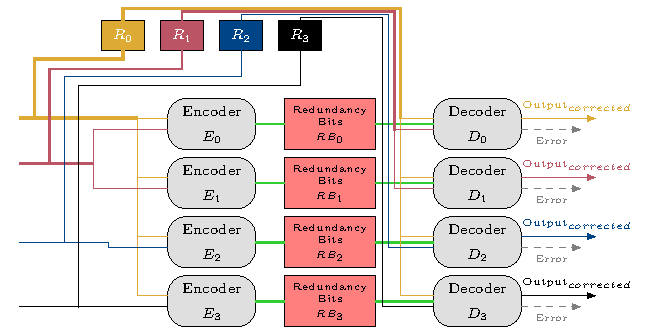
\includegraphics[page=1]{c6_group_composition/img/implem5_spaghetti.pdf}
    \caption{Strategy 5 -- Implementation idea}
    \label{fig:strategy_5_functionning}
\end{figure}

\begin{table}[t]
    \centering
    \footnotesize
    \caption{D-RI5CY Registers Details List for Strategy 5}
    \label{tab:strategy_5_register_info}
    % \setlength{\tabcolsep}{5pt}
    \begin{tabular}{@{}rccc@{}}
        \toprule
        Register Name                   & Module                                & Size   & \tableTwoLines{Strategy}{3} \\\midrule
        pc\_if\_o\_tag                  & \textcolor{red}{Fetch Stage}          & 1      & Gr1                         \\
        pc\_id\_o\_tag                  & \textcolor{red}{Instruction}          & 1      & Gr1                         \\\hdashline
        alu\_operand\_a\_ex\_o\_tag     &                                       & 1      & Gr4                         \\
        alu\_operand\_b\_ex\_o\_tag     &                                       & 1      & Gr5                         \\
        alu\_operand\_c\_ex\_o\_tag     &                                       & 1      & Gr6                         \\
        alu\_operator\_o\_mode          &                                       & 2      & Gr2 - Gr3                   \\
        check\_d\_o\_tag                &                                       & 1      & Gr9                         \\
        check\_s1\_o\_tag               &                                       & 1      & Gr7                         \\
        check\_s2\_o\_tag               & \textcolor{blue}{Instruction}         & 1      & Gr8                         \\
        is\_store\_post\_o\_tag         & \textcolor{blue}{Decode Stage}        & 1      & Gr10                        \\
        memory\_set\_o\_tag             &                                       & 1      & Gr11                        \\
        regfile\_alu\_waddr\_ex\_o\_tag &                                       & 5      & Gr5 - Gr9                   \\
        register\_set\_o\_tag           &                                       & 1      & Gr10                        \\
        store\_dest\_addr\_ex\_o\_tag   &                                       & 1      & Gr2                         \\
        store\_source\_ex\_o\_tag       &                                       & 1      & Gr3                         \\
        use\_store\_ops\_ex\_o          &                                       & 1      & Gr4                         \\\hdashline
        rf\_reg[0]                      &                                       & 1      & Gr12                          \\
        rf\_reg[1]                      &                                       & 1      & Gr12                          \\
        rf\_reg[2]                      & \textcolor{LimeGreen}{Register File}  & 1      & Gr12                          \\
        \ldots                          & \textcolor{LimeGreen}{Tag}            & \ldots & Gr12                          \\
        rf\_reg[30]                     &                                       & 1      & Gr12                          \\
        rf\_reg[31]                     &                                       & 1      & Gr12                          \\\hdashline
        rs1\_o\_tag                     & \textcolor{DarkOrange}{Execute Stage} & 1      & Gr35                            \\\hdashline
        tpr\_q                          & \textcolor{DarkRed}{Control and}      & 32     & Gr13 - Gr26 / Gr28 - Gr30                           \\
        tcr\_q                          & \textcolor{DarkRed}{Status Registers} & 32     & Gr13 - Gr34                          \\\hdashline
        data\_type\_q\_tag              &                                       & 2      & Gr36 - Gr37                            \\
        data\_we\_q\_tag                & \textcolor{magenta}{Load/Store}       & 1      & Gr39                            \\
        rdata\_offset\_q\_tag           & \textcolor{magenta}{Unit}             & 2      & Gr37 - Gr38                            \\
        rdata\_q\_tag                   &                                       & 4      & Gr35 - Gr36 / Gr38 - Gr39                            \\
        \bottomrule
    \end{tabular}
\end{table}

\begin{table}[t]
    \centering
    \footnotesize
    \caption{DIFT-related protected registers -- Strategy 5}
    \label{tab:strategy_5_groups}
    \begin{tabular}{@{}rccc@{}}
        \toprule
                 & \tableTwoLines{Number of}{protected bits} & \tableTwoLines{Number of}{redundancy bits} & \tableTwoLines{Number of}{parity bits} \\ \midrule
        Group 1  & 1                                         & 2                                          & 1                                      \\
        Group 2  & 1                                         & 2                                          & 1                                      \\
        Group 3  & 1                                         & 2                                          & 1                                      \\
        Group 4  & 1                                         & 2                                          & 1                                      \\
        Group 5  & 1                                         & 2                                          & 1                                      \\
        Group 6  & 2                                         & 3                                          & 1                                      \\
        Group 7  & 1                                         & 2                                          & 1                                      \\
        Group 8  & 1                                         & 2                                          & 1                                      \\
        Group 9  & 1                                         & 2                                          & 1                                      \\
        Group 10 & 1                                         & 2                                          & 1                                      \\
        Group 11 & 1                                         & 2                                          & 1                                      \\
        Group 12 & 5                                         & 4                                          & 1                                      \\
        Group 13 & 1                                         & 2                                          & 1                                      \\
        Group 14 & 1                                         & 2                                          & 1                                      \\
        Group 15 & 1                                         & 2                                          & 1                                      \\
        Group 16 & 1                                         & 2                                          & 1                                      \\
        Group 17 & 32                                        & 6                                          & 1                                      \\
        Group 18 & 1                                         & 2                                          & 1                                      \\
        Group 19 & 2                                         & 3                                          & 1                                      \\
        Group 20 & 2                                         & 3                                          & 1                                      \\
        Group 21 & 2                                         & 3                                          & 1                                      \\
        Group 22 & 2                                         & 3                                          & 1                                      \\
        Group 23 & 2                                         & 3                                          & 1                                      \\
        Group 24 & 2                                         & 3                                          & 1                                      \\
        Group 25 & 2                                         & 3                                          & 1                                      \\
        Group 26 & 3                                         & 3                                          & 1                                      \\
        Group 27 & 3                                         & 3                                          & 1                                      \\
        Group 28 & 2                                         & 3                                          & 1                                      \\
        Group 29 & 3                                         & 3                                          & 1                                      \\
        Group 30 & 3                                         & 3                                          & 1                                      \\
        Group 31 & 3                                         & 3                                          & 1                                      \\
        Group 32 & 3                                         & 3                                          & 1                                      \\
        Group 33 & 4                                         & 3                                          & 1                                      \\
        Group 34 & 1                                         & 2                                          & 1                                      \\
        Group 35 & 2                                         & 3                                          & 1                                      \\
        Group 36 & 2                                         & 2                                          & 1                                      \\
        Group 37 & 2                                         & 3                                          & 1                                      \\
        Group 38 & 4                                         & 3                                          & 1                                      \\ \midrule
        Total    & 103                                       & 101                                        & 38                                     \\
        \bottomrule
    \end{tabular}
\end{table}

\wip{modifier table \ref{tab:strategy_5_groups}}

%%%%%%%%%%%%%%%%%%%%%%%%%%%%%%%%%%%%%%%%%%%%%%%%%%%%%%%%%%%%%%%%%%%%%%%%%%%%%%%%%%%%%%%%%%%%%%%
\section{Experimental results}
\label{section:chap6_evaluation}

\begin{table}[t]
    \centering
    \footnotesize
    \caption{D-RI5CY Registers Details List}
    \label{tab:strategies_register_info}
    \setlength{\tabcolsep}{2pt}
    \begin{tabular}{@{}rccccccc@{}}
        \toprule
        Register Name                   & Module                                & Size   & \tableTwoLines{Strategy}{1} & \tableTwoLines{Strategy}{2} & \tableTwoLines{Strategy}{3} & \tableTwoLines{Strategy}{4} & \tableTwoLines{Strategy}{5} \\
        \midrule
        pc\_id\_o\_tag                  & \textcolor{red}{Instruction}          & 1      & Gr5                         & Gr1                         & Gr1                         & Gr1                         & Gr1                         \\
        pc\_if\_o\_tag                  & \textcolor{red}{Fetch Stage}          & 1      & Gr5                         & Gr1                         & Gr2                         & Gr2                         & Gr1                         \\\hdashline
        alu\_operand\_a\_ex\_o\_tag     &                                       & 1      & Gr5                         & Gr2                         & Gr3                         & Gr3                         & Gr4                         \\
        alu\_operand\_b\_ex\_o\_tag     &                                       & 1      & Gr5                         & Gr2                         & Gr4                         & Gr4                         & Gr5                         \\
        alu\_operand\_c\_ex\_o\_tag     &                                       & 1      & Gr5                         & Gr2                         & Gr5                         & Gr5                         & Gr6                         \\
        alu\_operator\_o\_mode          &                                       & 2      & Gr5                         & Gr2                         & Gr6                         & Gr6                         & Gr2 - Gr3                   \\
        check\_d\_o\_tag                &                                       & 1      & Gr5                         & Gr2                         & Gr7                         & Gr7                         & Gr9                         \\
        check\_s1\_o\_tag               &                                       & 1      & Gr5                         & Gr2                         & Gr8                         & Gr8                         & Gr7                         \\
        check\_s2\_o\_tag               & \textcolor{blue}{Instruction}         & 1      & Gr5                         & Gr2                         & Gr9                         & Gr9                         & Gr8                         \\
        is\_store\_post\_o\_tag         & \textcolor{blue}{Decode Stage}        & 1      & Gr5                         & Gr2                         & Gr10                        & Gr10                        & Gr10                        \\
        memory\_set\_o\_tag             &                                       & 1      & Gr5                         & Gr2                         & Gr11                        & Gr11                        & Gr11                        \\
        regfile\_alu\_waddr\_ex\_o\_tag &                                       & 5      & Gr4                         & Gr2                         & Gr12                        & Gr12                        & Gr5 - Gr9                   \\
        register\_set\_o\_tag           &                                       & 1      & Gr5                         & Gr2                         & Gr13                        & Gr13                        & Gr10                        \\
        store\_dest\_addr\_ex\_o\_tag   &                                       & 1      & Gr5                         & Gr2                         & Gr14                        & Gr14                        & Gr2                         \\
        store\_source\_ex\_o\_tag       &                                       & 1      & Gr5                         & Gr2                         & Gr15                        & Gr15                        & Gr3                         \\
        use\_store\_ops\_ex\_o          &                                       & 1      & Gr5                         & Gr2                         & Gr16                        & Gr16                        & Gr4                         \\\hdashline
        rf\_reg[0]                      &                                       & 1      & Gr3                         & Gr3                         & Gr17                        & Gr17                        & Gr12                        \\
        rf\_reg[1]                      &                                       & 1      & Gr3                         & Gr3                         & Gr17                        & Gr17                        & Gr12                        \\
        rf\_reg[2]                      & \textcolor{LimeGreen}{Register File}  & 1      & Gr3                         & Gr3                         & Gr17                        & Gr17                        & Gr12                        \\
        \ldots                          & \textcolor{LimeGreen}{Tag}            & \ldots & Gr3                         & Gr3                         & Gr17                        & Gr17                        & Gr12                        \\
        rf\_reg[30]                     &                                       & 1      & Gr3                         & Gr3                         & Gr17                        & Gr17                        & Gr12                        \\
        rf\_reg[31]                     &                                       & 1      & Gr3                         & Gr3                         & Gr17                        & Gr17                        & Gr12                        \\\hdashline
        rs1\_o\_tag                     & \textcolor{DarkOrange}{Execute Stage} & 1      & Gr5                         & Gr4                         & Gr18                        & Gr18                        & Gr35                        \\\hdashline
        tcr\_q                          & \textcolor{DarkRed}{Control and}      & 32     & Gr1                         & Gr5                         & Gr19                        & Gr19 - Gr26                 & Gr13 - Gr26 / Gr28 - Gr30   \\
        tpr\_q                          & \textcolor{DarkRed}{Status Registers} & 32     & Gr2                         & Gr6                         & Gr20                        & Gr27 - Gr34                 & Gr13 - Gr34                 \\\hdashline
        data\_type\_q\_tag              &                                       & 2      & Gr5                         & Gr7                         & Gr21                        & Gr35                        & Gr36 - Gr37                 \\
        data\_we\_q\_tag                & \textcolor{magenta}{Load/Store}       & 1      & Gr5                         & Gr7                         & Gr22                        & Gr36                        & Gr39                        \\
        rdata\_offset\_q\_tag           & \textcolor{magenta}{Unit}             & 2      & Gr5                         & Gr7                         & Gr23                        & Gr37                        & Gr37 - Gr38                 \\
        rdata\_q\_tag                   &                                       & 4      & Gr5                         & Gr7                         & Gr24                        & Gr38                        & Gr35 - Gr36 / Gr38 - Gr39   \\
        \bottomrule
    \end{tabular}
\end{table}


\begin{table}[t]
    \centering
    \footnotesize
    \caption{Registers by Strategy (SECDED count): Summary of Number and Size}
    \label{tab:strategies_summary}
    \begin{tabular}{rcc}
        \toprule
        Strategy            & Number of Registers & Number of Bits \\
        \midrule
        Baseline -- D-RI5CY & 55                  & 127            \\
        Strategy 1          & 65                  & 157            \\
        Strategy 2          & 69                  & 164            \\
        Strategy 3          & 103                 & 215            \\
        Strategy 4          & 131                 & 266            \\
        Strategy 5          & 133                 & 280            \\
        \bottomrule
    \end{tabular}
\end{table}


%%%%%%%%%%%%%%%%%%%%%%%%%%%%%%%%%%%%%%%%%%%%%%%%%%%%%%%%%%%%%%%%%%%%%%%%%%%%%%%%%%%%%%%%%%%%%%%
\section{Discussion}
\label{section:chap6_discussion}

%%%%%%%%%%%%%%%%%%%%%%%%%%%%%%%%%%%%%%%%%%%%%%%%%%%%%%%%%%%%%%%%%%%%%%%%%%%%%%%%%%%%%%%%%%%%%%%
\section{Summary}


%%%%%%%%%%%%%%%%%%%%%%%%%%%%%%%%%%%%%%%%%%%%%%%%%%%%%%%%%%%%%%%%%%%%%%%%%%%%%%%%%%%%%%%%%%%%%%%